\chapter{Manuale Utente}
\label{chap:manuale_utente}
Questo capitolo ha lo scopo di discutere e presentare le varie schermate dell'applicazione e di fornire una guida sull'utilizzo di quest'ultima, mettendo in evidenza cosa rappresenta ogni schermata. In particolare, saranno analizzati i vari elementi di ogni schermata e le varie rotte di navigazione che vengono offerte dalle varie parti dell'applicazione. Verrà inoltre presentato il flusso dell'applicazione, vale a dire cosa è stato progettato che l'utente veda e in che ordine dal primo avvio fino all'utilizzo quotidiano e il motivo per il quale è stato adottato tale flusso.

\section{Prerequisiti}
Per poter utilizzare l'applicazione, almeno per quanto riguarda Android, è necessario uno smartphone con una versione di android con \textbf{API di livello almeno 19}\footnote{\url{source.android.com/setup/start/build-numbers}}, ovvero con almeno \textbf{Android 4.4 KitKat}, tuttavia è consigliato utilizzare almeno \textbf{Android 5.0 Lollipop} per via di alcune funzionalità che potrebbero non funzionare ugualmente bene su version anteriori. Considerando gli sviluppi attuali del sistema operativo è ragionevole pensare tutti i dispositivi Android supportino almeno Lollipop, che è stata la rivoluzione di casa Google in termini di sistema operativo, modificando aspetti legati all'esecuzione di applicazioni e mettendo in pratica il material design. Per quanto riguarda iOS, la versione minima supportata da Flutter è \textbf{iOS 9.0}\footnote{\url{flutter.dev/docs/development/tools/sdk/release-notes/supported-platforms}}.

\newpage
\section{On-Boarding}
Al primo avvio dell'applicazione l'utente verrà accolto da una brevissima introduzione su cosa fa l'applicazione e come si propone di farlo. Questa introduzione è estremamente riassuntiva e ha lo scopo di evitare che l'utente si trovi davanti da subito una schermata complicata e che potrebbe creare confusione a prima vista. Possiamo vedere nella Figura \ref{fig:on_boarding} tale schermata, composta da tre pagine opportunamente animate e curate esteticamente; questa è la prima impressione che l'applicazione darà all'utente ed è quindi importante che queste pagine siano curate nei minimi dettagli.

\begin{figure}[h!]
\centering
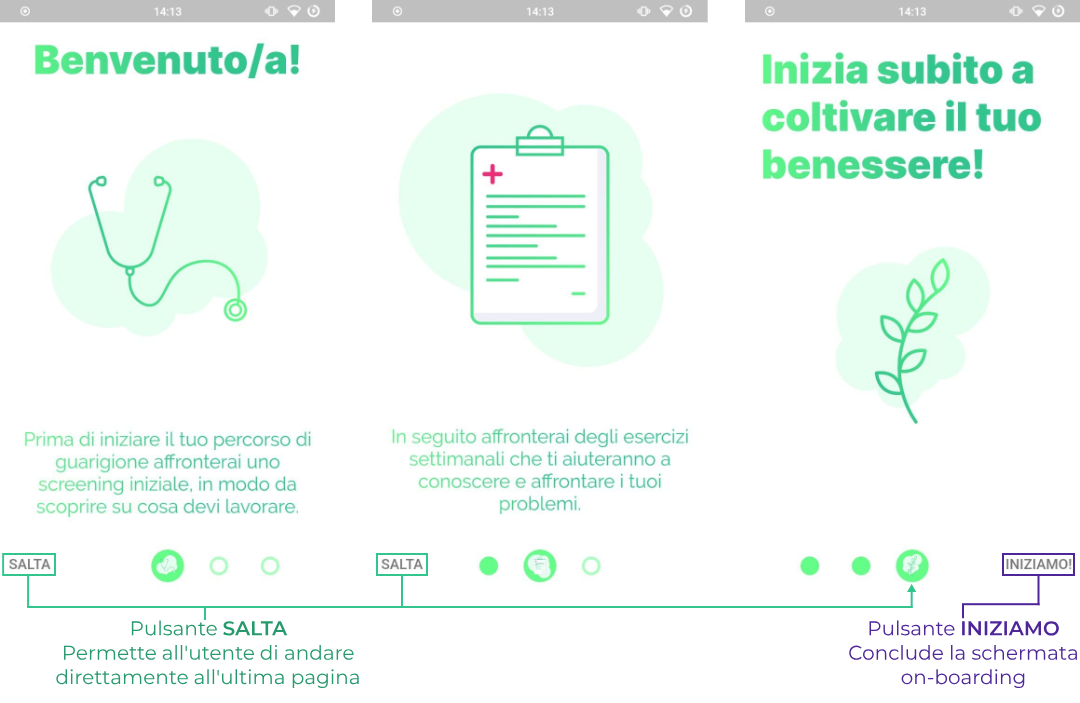
\includegraphics[width=\textwidth]{img/on_boarding}
\caption{Schermata on-boarding}
\label{fig:on_boarding}
\end{figure}

\newpage
\section{Presentazione tutor}
Conclusa la schermata on-boarding, l'utente verrà accolto da una schermata di introduzione delle tutor di psicologia, accompagnata da video, nella quale ciascuna tutor si presenterà all'utente, spiegherà di che sintomatologia si occupa e come sarà costruito il proprio percorso. In questa fase c'è anche una spiegazione più dettagliata su come funziona l'applicazione, come sono erogati gli esercizi settimanali e le domande giornaliere e cosa comprendono. Possiamo vedere in dettaglio la schermata di presentazione nella Figura \ref{fig:presentazione_tutor}.

\begin{figure}[h!]
\centering
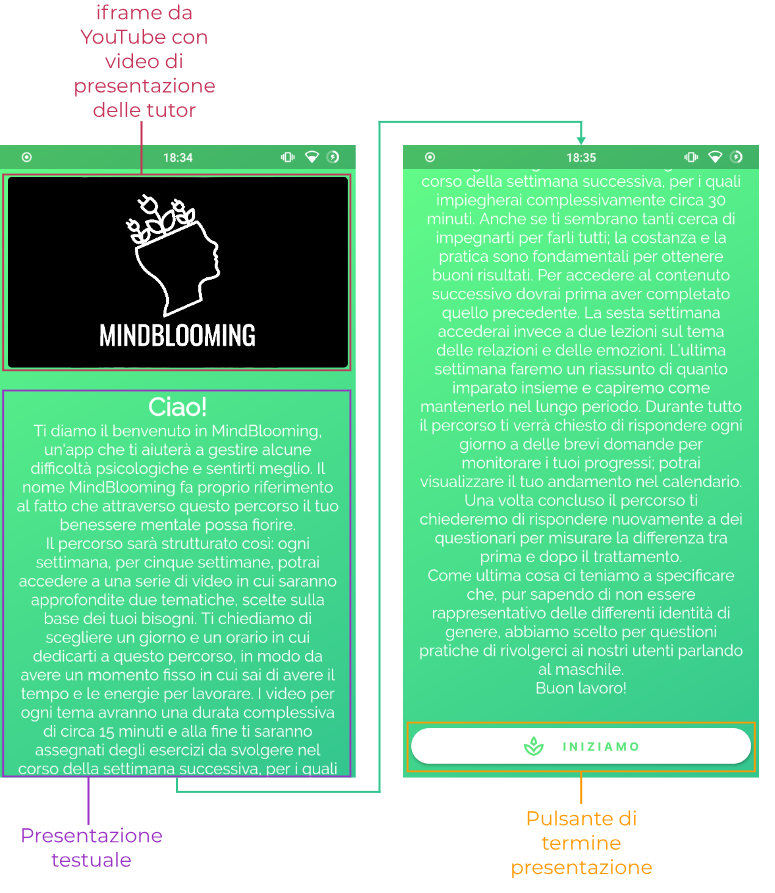
\includegraphics[width=0.85\textwidth]{img/presentazione_tutor}
\caption{Schermata presentazione tutor}
\label{fig:presentazione_tutor}
\end{figure}

\newpage
\section{Screening}
\label{section:screening}
A questo punto l'utente è pronto ad eseguire gli screening iniziali per poter individuare le eventuali patologie di cui soffre. Come possiamo vedere nella Figura \ref{fig:screening}, all'utente verrà presentata una lista con le varie sezioni dello screening, che vanno da alcuni criteri di inclusione fino agli screening veri e propri di ogni patologia. Possiamo osservare inoltre come per poter accedere ad una sezione, l'utente deve prima completare la precedente. Inoltre, all'utente sarà visibile anche la presentazione generale di prima, consultabile in qualsiasi momento.

\begin{figure}[h!]
\centering
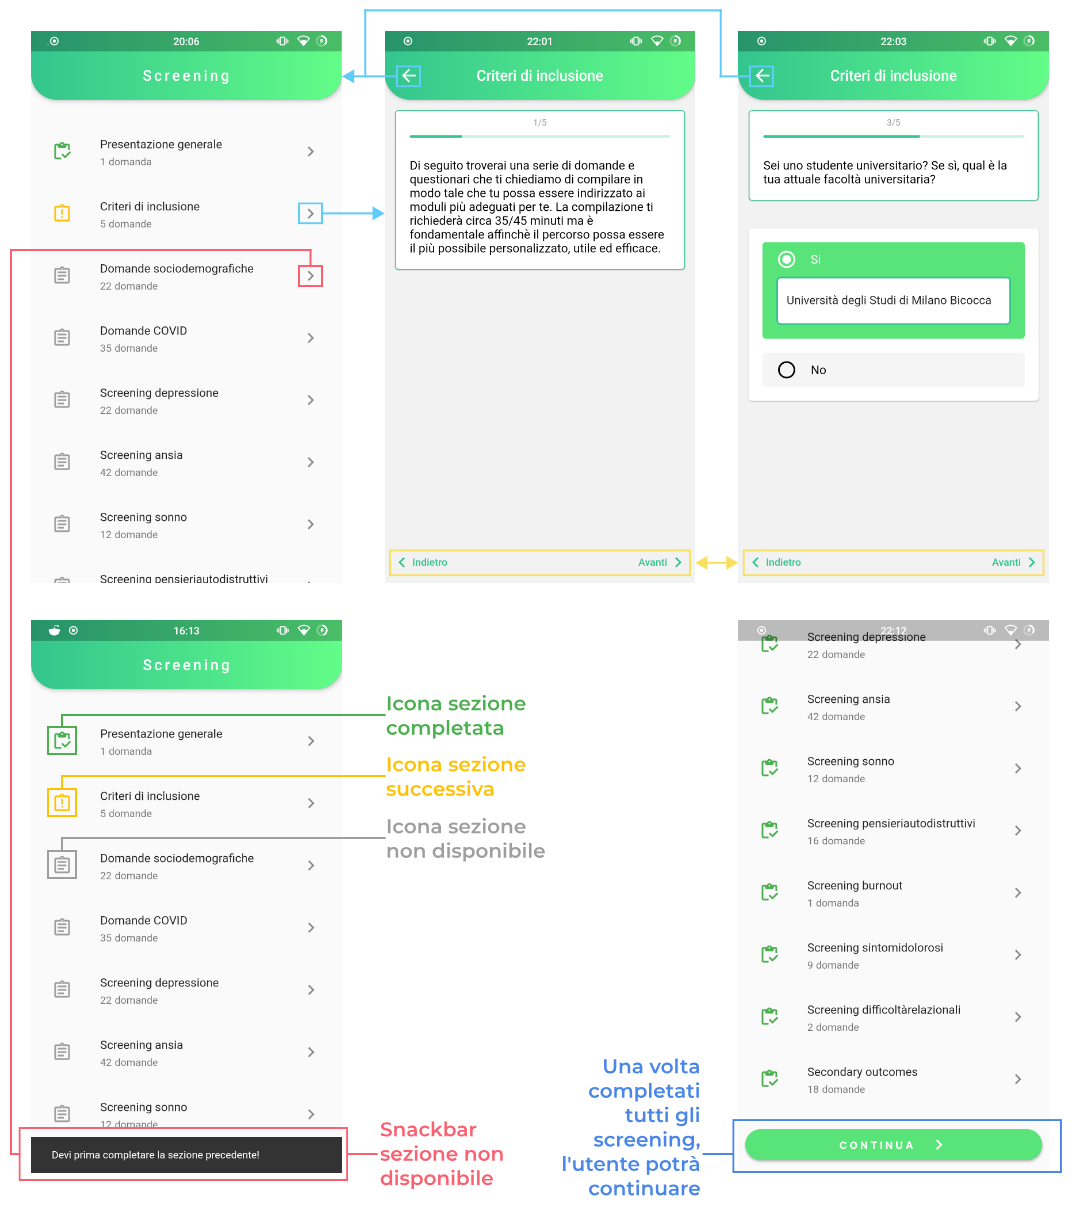
\includegraphics[width=0.88\textwidth]{img/screening}
\caption{Schermata Screening}
\label{fig:screening}
\end{figure}

\section{Risultati}
Una volta completati tutti gli screenig, l'utente potrà procedere verso la schermata dei risultati, visibile in Figura \ref{fig:risultati}, in cui verranno comunicati i disturbi rilevati, se ve ne sono, con un'eventuale descrizione di questi. Se l'algoritmo di screening individua esattamente due patologie su cui lavorare, l'utente da questa schermata potrà andare direttamente alla schermata finale delle impostazioni, mentre se l'algoritmo ne identifica solo uno oppure ne identifica più di due senza poter scegliere una priorità, l'utente verrà condotto ad una schermata di scelta delle patologie. Se nessuna patologia viene rilevata dall'algoritmo, l'utente andrà direttamente alla schermata di scelta delle patologie, dove potrà comunque sceglierne due.

\begin{figure}[h!]
\centering
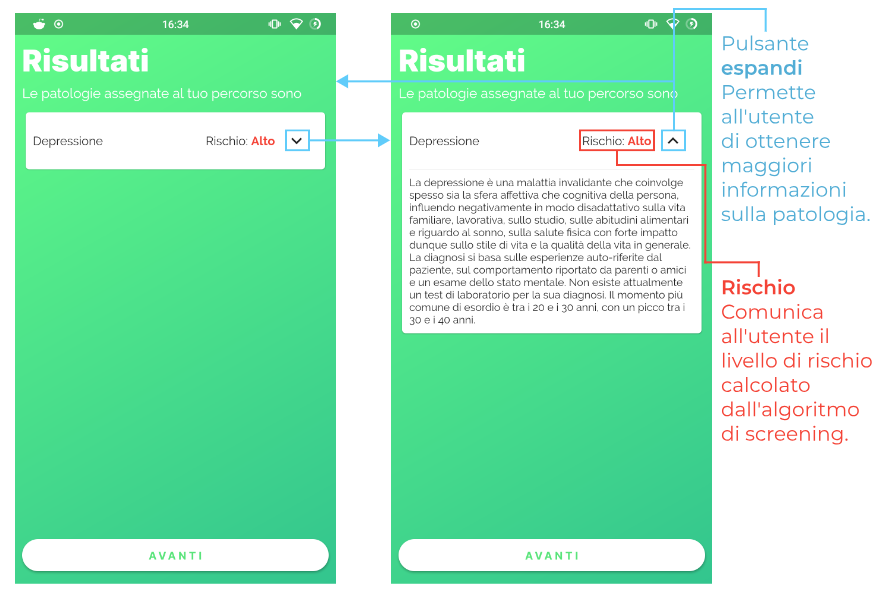
\includegraphics[width=\textwidth]{img/risultati}
\caption{Schermata Risultati}
\label{fig:risultati}
\end{figure}

\newpage
\section{Selezione patologie}
Come detto prima, nel caso l'algoritmo non identifichi due patologie o nel caso non fosse possibile definire delle priorità tra quelle identificate, all'utente verrà presentata anche la schermata di scelta delle patologie che, come è visibile nella Figura \ref{fig:scelta_patologie}, è molto simile alla precedente, ma permette di selezionare effettivamente le patologie \textit{(fino ad arrivare a due patologie complessive tra scelte dall'algoritmo e scelte dall'utente)}.

\begin{figure}[h!]
\centering
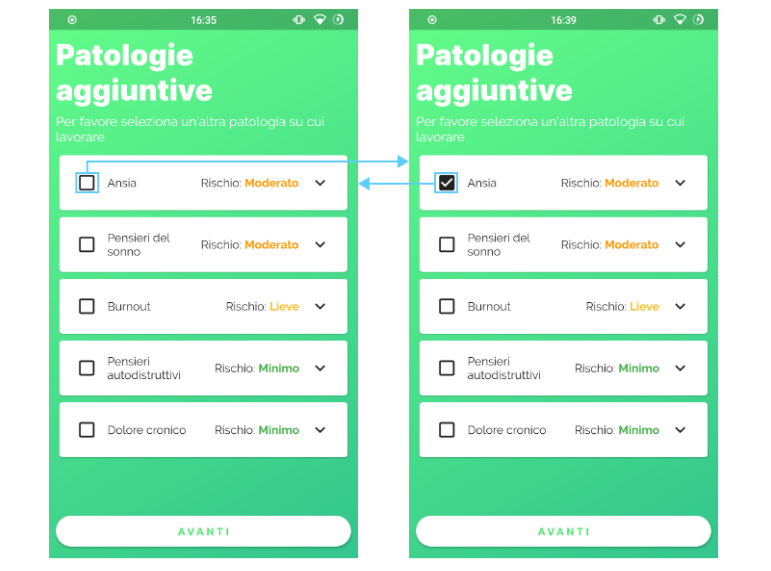
\includegraphics[width=\textwidth]{img/scelta_patologie}
\caption{Schermata Selezione patologie}
\label{fig:scelta_patologie}
\end{figure}

\newpage
\section{Impostazioni iniziali}
\label{section:impostazioni}
Una volta scelte le patologie, come è osservabile nella Figura \ref{fig:settaggi}, l'utente potrà scegliere alcune impostazioni iniziali come l'orario al quale ricevere la notifica dello screening giornaliero \textit{(daily screening)} e un eventuale 'compagno di viaggio', ovvero una piantina che mostri l'andamento del percorso curativo e che crescerà man mano che l'utente completa gli esercizi \textit{(questa funzionalità fa parte degli sviluppi futuri tuttavia)}. Conclusa questa schermata l'utente accederà alla homepage. È possibile osservare come i metodi di selezione dell'orario e della piantina siano molto basilari e semplici in modo che sia subito evidente come utilizzarli.

\begin{figure}[h!]
\centering
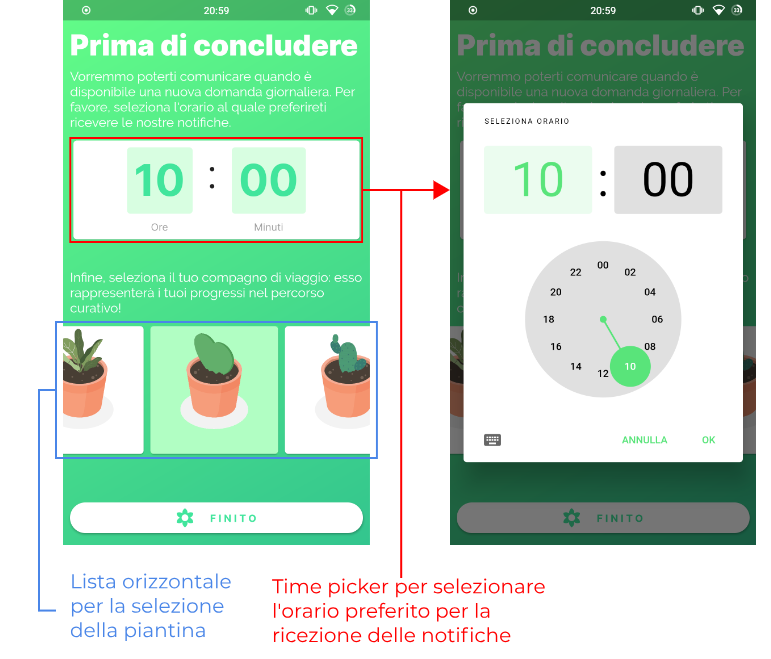
\includegraphics[width=\textwidth]{img/settaggi}
\caption{Schermata impostazioni iniziali}
\label{fig:settaggi}
\end{figure}

\newpage
\section{Homepage}
La homepage, la schermata che l'utente vedrà appena aperta l'applicazione una volta conclusa la fase di screening, è composta, come è osservabile in Figura \ref{fig:homepage}, da un calendario che mostrerà all'utente le scadenze dei vari esercizi e daily screening e dalla piantina che mostrerà l'andamento del suo percorso. In particolare, il calendario evidenzierà gli esercizi in scadenza nel giorno corrente e quelli completati.

\begin{figure}[h!]
\centering
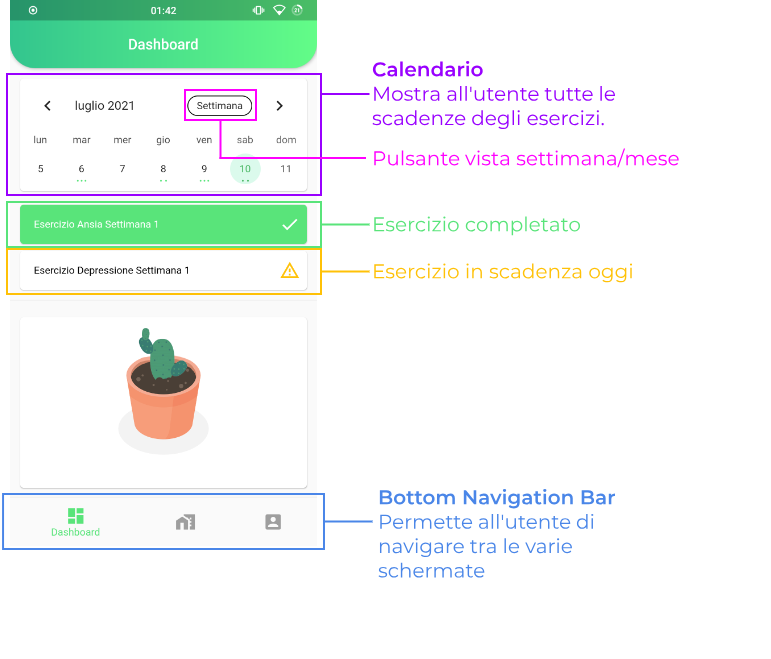
\includegraphics[width=\textwidth]{img/homepage}
\caption{Schermata Homepage}
\label{fig:homepage}
\end{figure}

\newpage
\section{Esercizi}
In questa schermata l'utente può visualizzare gli esercizi disponibili e rivedere quelli già completati, in modo che l'utente abbia sempre accesso alle risorse multimediali messe a disposizione dall'applicazione. Come mostrato in \autoref{fig:schermata_esercizi}, la schermata contiene uno switch che permette all'utente di vedere gli esercizi disponibili o quelli già completati. Accedendo ad un esercizio, all'utente verrà presentata una schermata di sezioni, ognuna delle quali contenente delle domande, come quella vista nella \autoref{section:screening}.

\begin{figure}[h!]
\centering
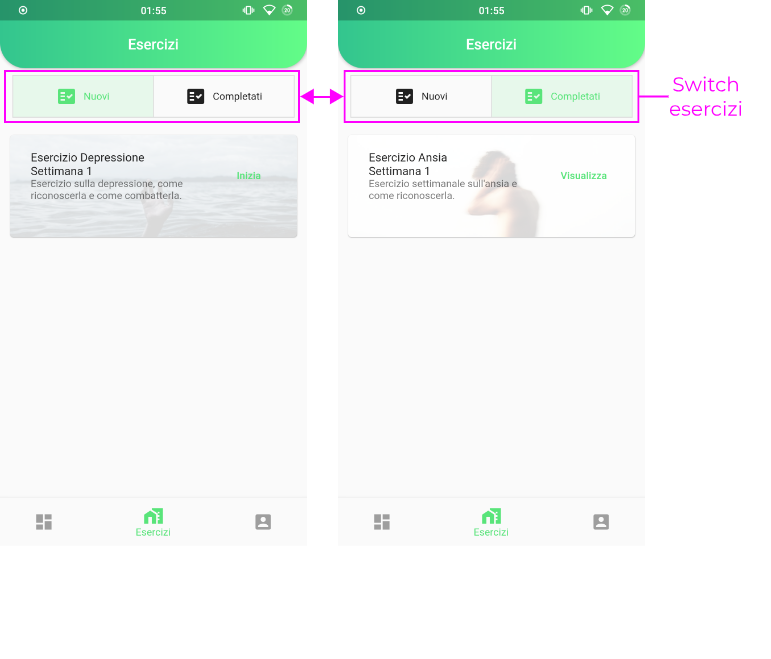
\includegraphics[width=\textwidth]{img/schermata_esercizi}
\caption{Schermata Esercizi}
\label{fig:schermata_esercizi}
\end{figure}

\newpage
\section{Profilo}
Infine, nella schermata profilo l'utente potrà modificare le proprie impostazioni, ovvero, come visibile in \autoref{fig:profilo}, cambiare l'orario delle notifiche e la propria piantina. Notiamo che gli widget utilizzati per la modifica di queste impostazioni sono i medesimi utilizzate nell'impostazione iniziale mostrata nella \autoref{section:impostazioni}.

\begin{figure}[h!]
\centering
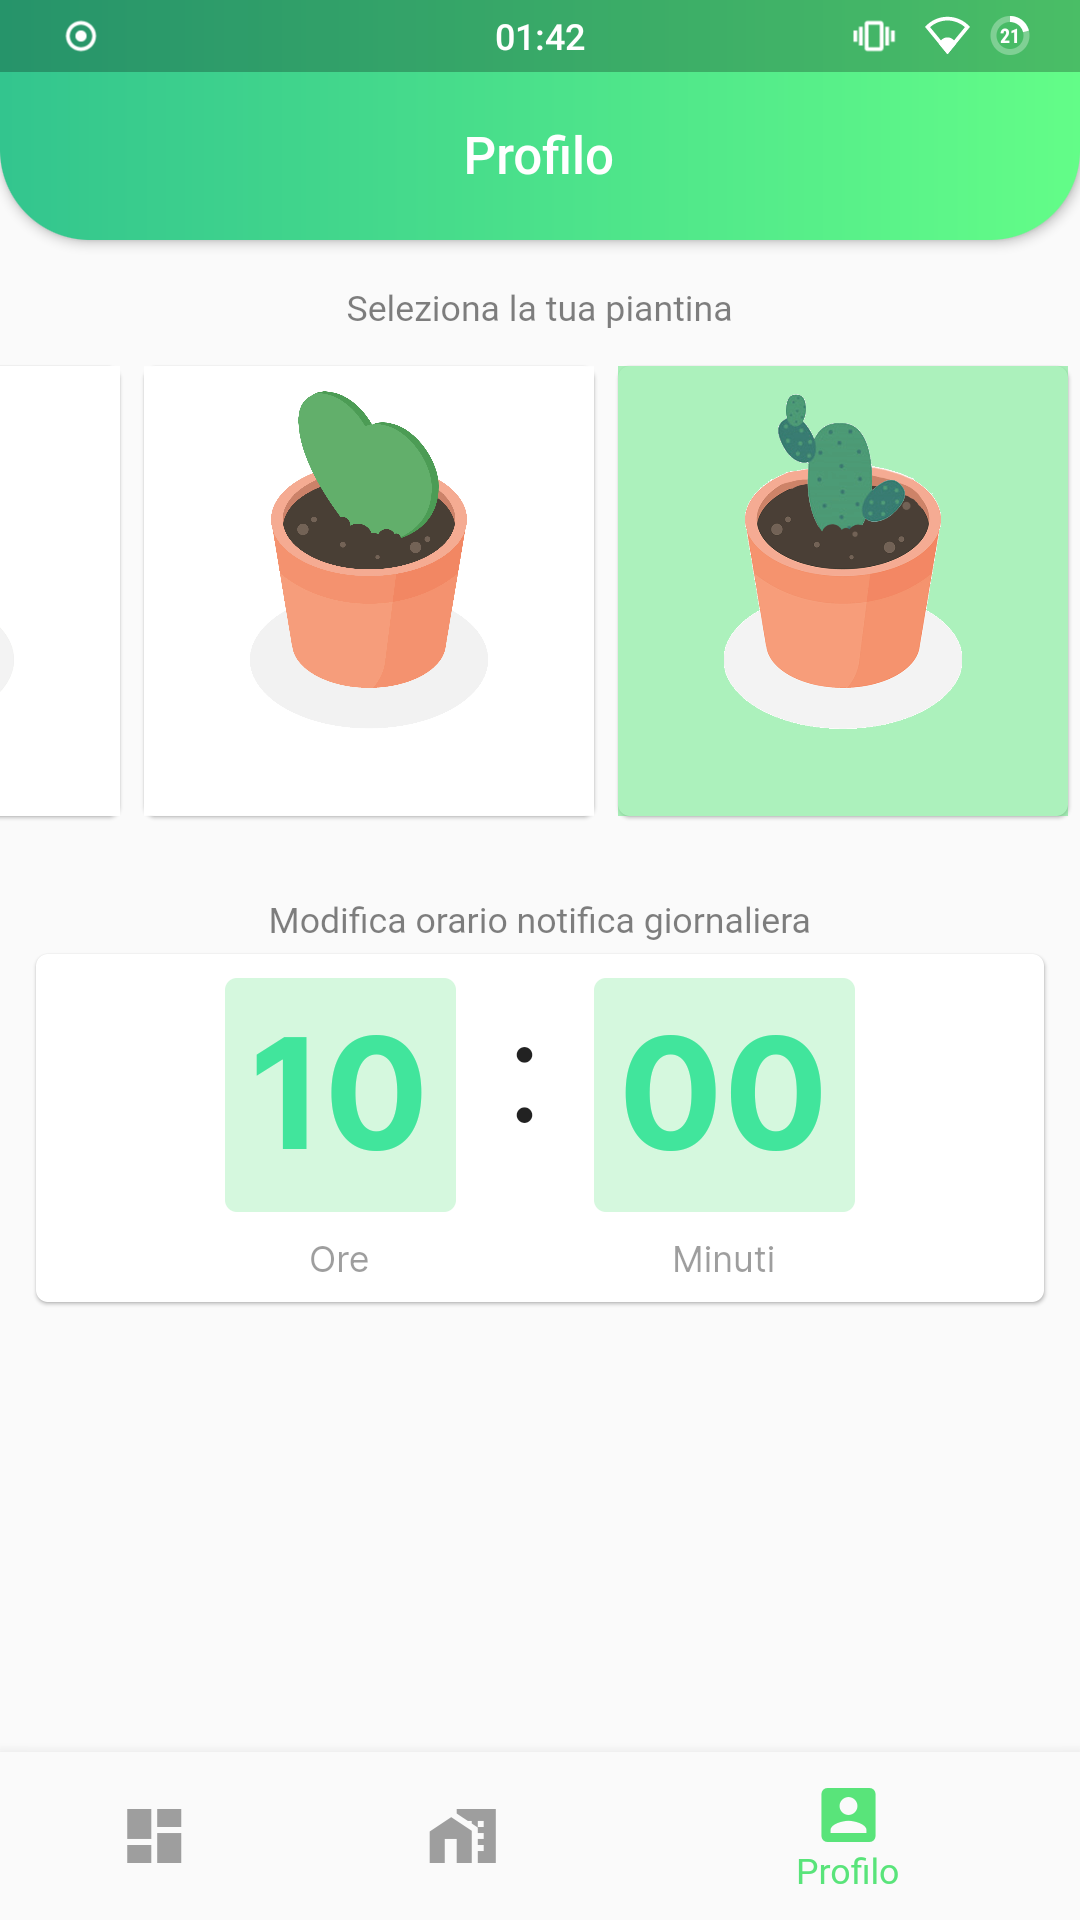
\includegraphics[width=0.5\textwidth]{img/profilo}
\caption{Schermata Profilo}
\label{fig:profilo}
\end{figure}